\documentclass{article} % Use the article class for a simple document
\usepackage{amsmath}    % For enhanced math environments
\usepackage{amsfonts}   % For mathematical fonts
\usepackage{amssymb}    % For mathematical symbols
\usepackage{array}      % Enhances array and tabular environments
\usepackage{booktabs}   % For better looking tables (optional, but recommended)
\usepackage{graphicx}
\usepackage{tikz}

\title{Function Translations}
\author{A. I. Assistant}
\date{\today}

\begin{document}

\maketitle % Displays the title, author, and date

\section*{Function Translation Rules}

\subsection*{Transformation Rules}
The following table summarizes the rules for vertical translation of a function $y = f(x)$.

\begin{table}[h!]
\centering
\caption{Translation Rules}
\label{tab:vertical_translation}
\begin{tabular}{|c|c|c|c|}
\hline
\textbf{Function} & \textbf{Vertical Translation} & \textbf{Result} & \textbf{Point} \\
\hline
$y = f(x)$ & \textbf{Upward} by $k$ units & $y = f(x) + k$ & $(x, y + k)$ \\
\hline
$y = f(x)$ & \textbf{Downward} by $k$ units & $y = f(x) - k$ & $(x, y - k)$ \\
\hline
$y = f(x)$ & \textbf{Right} by $h$ units & $y = f(x - h)$ & $(x - h, y)$ \\
\hline
$y = f(x)$ & \textbf{Left} by $h$ units & $y = f(x + h)$ & $(x + h, y)$ \\
\hline
$y = f(x)$ & \textbf{Stretch} by $h$ units & $y = f(x - h)$ & $(x - h, y)$ \\
\hline
$y = f(x)$ & \textbf{LeSft} by $h$ units & $y = f(x + h)$ & $(x + h, y)$ \\
\hline
\end{tabular}
\end{table}

\subsection*{Parent Translation}
The following table summarizes the rules for horizontal translation of a function $y = f(x)$.

\begin{table}[h!]
\centering
\caption{Translating $f(x)=x^2$}
\label{tab:vertical_translation}
\begin{tabular}{|c|c|c|c|}
\hline
\textbf{Function} & \textbf{Vertical Translation} & \textbf{Result} & \textbf{Point} \\
\hline
$y = x^2$ & \textbf{Upward} by $k$ units & $y = x^2 + k$ & $(x, y + k)$ \\
\hline
$y = x^2$ & \textbf{Downward} by $k$ units & $y = x^2 - k$ & $(x, y - k)$ \\
\hline
$y = x^2$ & \textbf{Right} by $h$ units & $y = (x - h)^2$ & $(x - h, y)$ \\
\hline
$y = x^2$ & \textbf{Left} by $h$ units & $y = (x + h)^2$ & $(x + h, y)$ \\
\hline
\end{tabular}
\end{table}

\section*{Quadratic Function Transformations}

% The tabular environment uses fixed-width columns (p{}) to ensure text wrapping.
% The vertical height is enforced using \rule{0pt}{5cm} inside the second data row.
\begin{tabular}{|>{\centering\arraybackslash}p{2.5cm}|p{4cm}|p{4cm}|>{\centering\arraybackslash}p{2.5cm}|}
\hline
\textbf{Function} & \textbf{Vertical Translation} & \textbf{Resulting Equation} & \textbf{Transformed Point} \\
\hline
$y = x^2$ & Upward by $k$ units & $y = x^2 + k$ & $(x, y + k)$ \\
\hline
% This row contains the large vertical gap, enforced by \rule{0pt}{5cm}
$y = x^2$ & \rule{0pt}{5cm}Downward by $k$ units & $y = x^2 - k$ & $(x, y - k)$ \\
\hline
\end{tabular}

\section*{Quadratic Function Transformations}

% The tabular environment uses fixed-width columns (p{}) to ensure text wrapping.
% The vertical height is enforced using \rule{0pt}{5cm} inside the second data row.
Convert each of the following Transformations from function notation to words
\begin{tabular}{|>{\centering\arraybackslash}p{3cm}|p{3cm}|p{3cm}|>{\centering\arraybackslash}p{3cm}|}
\hline
$y = \displaystyle\frac{1}{2}f(x-1)+2$ & $y=5f(-x)+3$ & $y=-2f(x+1)-2$ & $y=f(x-3)+4$ \\
% This row contains the large vertical gap, enforced by \rule{0pt}{5cm}
& \rule{0pt}{5cm}& &  \\
\hline
\end{tabular}

\vspace{4cm}
\section*{Quadratic Function Transformations}

% The tabular environment uses fixed-width columns (p{}) to ensure text wrapping.
% The vertical height is enforced using \rule{0pt}{5cm} inside the second data row.
If $(3,4)$ is a point on the graph $f(x)$, what ordered pair must also be \\ on the graph of $y$ using the same Transformation from above \\
\begin{tabular}{|>{\centering\arraybackslash}p{3cm}|p{3cm}|p{3cm}|>{\centering\arraybackslash}p{3cm}|}
\hline
$y = \displaystyle\frac{1}{2}f(x-1)+2$ & $y=5f(-x)+3$ & $y=-2f(x+1)-2$ & $y=f(x-3)+4$ \\
% This row contains the large vertical gap, enforced by \rule{0pt}{5cm}
& \rule{0pt}{5cm}& &  \\
\hline
\end{tabular}


\section*{Quadratic Function Transformations}
\begin{minipage}[c]{0.40\textwidth} % Minipage for all graphs
    \centering

    % === GRAPH 1 ===
    Adjust $y=f(x)$ with transformation $y=2f(x)$
    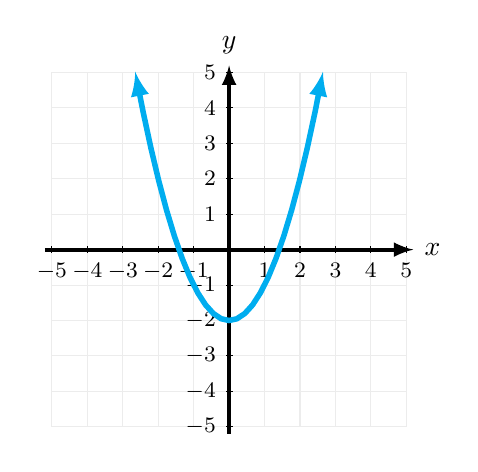
\begin{tikzpicture}
	[
		scale=0.45,
		vector style/.style={->, very thick}
	]
    \draw[gray!15,step=1cm] (-5,-5) grid (5,5);
        \draw[line width=0.5mm, -latex] (-5.2,0) -- (5.2,0) node[right] {$x$};
        \foreach \x in {-5,-4,-3,-2,-1,1,2,3,4,5} \draw (\x,.1)--(\x,-.1) node[below] {\footnotesize $\x$};
        \draw[line width=0.5mm,  -latex] (0,-5.2) -- (0,5.2) node[above] {$y$};
        \foreach \y in {-5,-4,-3,-2,-1,1,2,3,4,5} \draw (.1,\y)--(-.1,\y) node[left] {\footnotesize $\y$};
        \draw[cyan,line width=2pt,latex-latex] plot[domain= -2.65:2.65] (\x,{\x*\x-2});
    \end{tikzpicture}

    \vspace{0.5cm} % Add some space between graphs

    % === GRAPH 2 ===
    Adjust $y=h(x)$ with transformation $y=h(x-3)$
    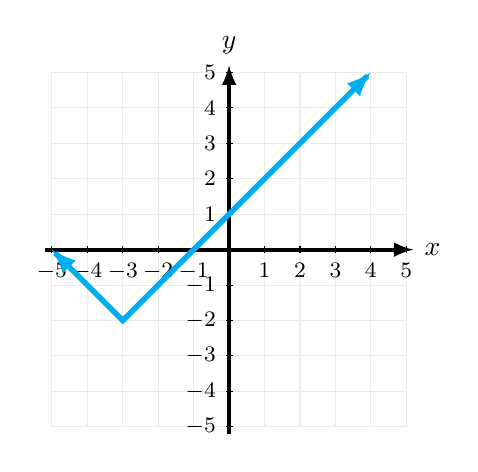
\begin{tikzpicture}
	[
		scale=0.45,
		vector style/.style={->, very thick}
	]
    \draw[gray!15,step=1cm] (-5,-5) grid (5,5);
        \draw[line width=0.5mm, -latex] (-5.2,0) -- (5.2,0) node[right] {$x$};
        \foreach \x in {-5,-4,-3,-2,-1,1,2,3,4,5} \draw (\x,.1)--(\x,-.1) node[below] {\footnotesize $\x$};
        \draw[line width=0.5mm,  -latex] (0,-5.2) -- (0,5.2) node[above] {$y$};
        \foreach \y in {-5,-4,-3,-2,-1,1,2,3,4,5} \draw (.1,\y)--(-.1,\y) node[left] {\footnotesize $\y$};
        \draw[cyan,line width=2pt,latex-latex] plot[domain= -5:4, samples=100] (\x,{abs(\x + 3) - 2});
    \end{tikzpicture}

\end{minipage}
\hfill
\begin{minipage}[c]{0.40\textwidth} % Minipage for all graphs
    \centering

    % === GRAPH 4 ===
    Adjust $y=g(x)$ with transformation $y=-g(x)$
    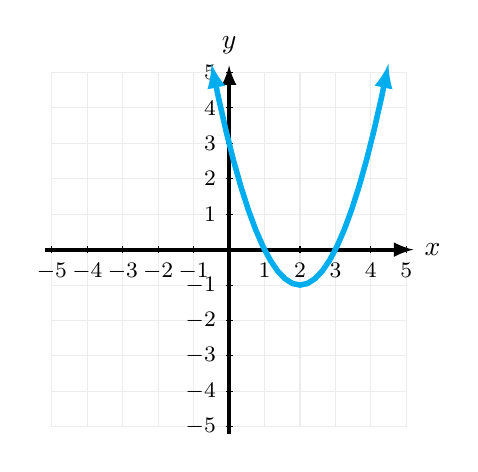
\begin{tikzpicture}
	[
		scale=0.45,
		vector style/.style={->, very thick}
	]
    \draw[gray!15,step=1cm] (-5,-5) grid (5,5);
        \draw[line width=0.5mm, -latex] (-5.2,0) -- (5.2,0) node[right] {$x$};
        \foreach \x in {-5,-4,-3,-2,-1,1,2,3,4,5} \draw (\x,.1)--(\x,-.1) node[below] {\footnotesize $\x$};
        \draw[line width=0.5mm,  -latex] (0,-5.2) -- (0,5.2) node[above] {$y$};
        \foreach \y in {-5,-4,-3,-2,-1,1,2,3,4,5} \draw (.1,\y)--(-.1,\y) node[left] {\footnotesize $\y$};
        \draw[cyan,line width=2pt,latex-latex] plot[domain= -0.5:4.5] (\x,{((\x-2)^2) - 1});
    \end{tikzpicture}

    \vspace{0.5cm} 

    % === GRAPH 5 ===
    Adjust $y=k(x)$ with transformation $y=-k(x)-3$
    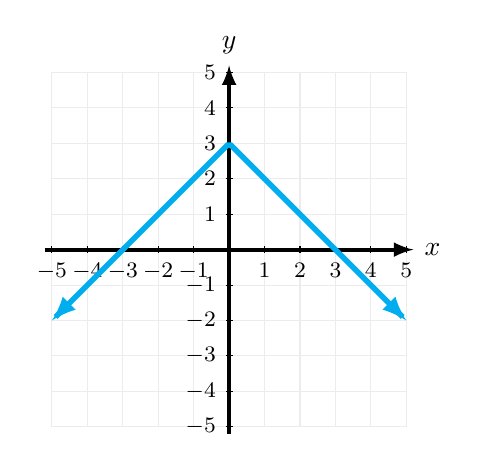
\begin{tikzpicture}
	[
		scale=0.45,
		vector style/.style={->, very thick}
	]
    \draw[gray!15,step=1cm] (-5,-5) grid (5,5);
        \draw[line width=0.5mm, -latex] (-5.2,0) -- (5.2,0) node[right] {$x$};
        \foreach \x in {-5,-4,-3,-2,-1,1,2,3,4,5} \draw (\x,.1)--(\x,-.1) node[below] {\footnotesize $\x$};
        \draw[line width=0.5mm,  -latex] (0,-5.2) -- (0,5.2) node[above] {$y$};
        \foreach \y in {-5,-4,-3,-2,-1,1,2,3,4,5} \draw (.1,\y)--(-.1,\y) node[left] {\footnotesize $\y$};
        \draw[cyan,line width=2pt,latex-latex] plot[domain= -5:5, samples=100] (\x,{-1*abs(\x) + 3});
    \end{tikzpicture}

    \vspace{0.5cm} 

    

\end{minipage}
\end{document}